\section{Sintonía PID Analógica por Prueba y Error}

\subsection{Ajustar empíricamente el PID buscando sobrepaso máximo del \texorpdfstring{$10\%$}{10\%}}

El método de prueba y error consiste en modificar empíricamente $K_p$, $T_i$ y $T_d$ hasta cumplir las especificaciones.  
En particular, buscamos que el sobrepaso máximo no supere el $10\%$.

Para ello, debemos tener en cuenta lo siguiente:
\begin{itemize}
	\item $K_p$ acelera la respuesta pero aumenta oscilación y sobrepaso.
	\item $T_i$ reduce el error en régimen y puede acortar el asentamiento, pero en exceso produce oscilación.
	\item $T_d$ atenúa el sobrepaso (amortigua) a costa de mayor sensibilidad al ruido.
\end{itemize}

\subsection{Analizar el efecto del control}

Se implementó un \textit{script} en \textsc{Matlab} que permite probar varias combinaciones de parámetros y registrar las métricas de cada intento.


\begin{strip}

	\vspace{-\baselineskip} % ajusta si ves demasiado aire arriba
	\noindent
	\begin{minipage}{0.98\textwidth}
		
	\begin{lstlisting}[language=Matlab, style=matlabstyle]
		function results = diseno_pid(G, filename)
		% diseno_pid - Bucle interactivo para sintonia PID y selección del mejor ensayo
		%
		% Uso:
		%   [Kp, Ti, Td] = diseno_pid(G, 'log_pid.mat', OSd, trd, tsd)
		
		if nargin < 2
		filename = 'log_pid.mat';
		end
		if nargin < 3, OSd = []; end
		if nargin < 4, trd = []; end
		if nargin < 5, tsd = []; end
		
		results = struct([]);
		if exist(filename,'file')
		S = load(filename);
		if isfield(S,'results'), results = S.results; end
		end
		k_iter = numel(results) + 1;
	\end{lstlisting}
	
\end{minipage}
\vspace{-\baselineskip} % ajusta si ves aire abajo
\end{strip}

\begin{strip}
\vspace{-\baselineskip} % ajusta si ves demasiado aire arriba
\noindent
\begin{minipage}{0.98\textwidth}


	\begin{lstlisting}[language=Matlab, style=matlabstyle, caption={Función para diseño PID por prueba y error.}, label={lst:disenoPID}]
		while true
		fprintf('\n--- Parametros PID ---\n');
		Kp = input('Kp: ');
		Td = input('Td: ');
		Ti = input('Ti: ');
		numC = Kp*[Ti*Td, Ti, 1];
		denC = [Ti, 0];
		C = tf(numC, denC);
		cl = feedback(C*G, 1);
		
		info = stepinfo(cl);
		OS = info.Overshoot;
		tr = info.RiseTime;
		ts = info.SettlingTime;
		
		% guardar en struct
		results(k_iter).Kp = Kp;
		results(k_iter).Ti = Ti;
		results(k_iter).Td = Td;
		results(k_iter).Overshoot = OS;
		results(k_iter).RiseTime = tr;
		results(k_iter).SettlingTime = ts;
		save(filename,'results');
		k_iter = k_iter + 1;
		
		resp = input('Continuar? [s/n]: ','s');
		if isempty(resp) || any(lower(resp(1)) == ['n','q'])
		disp('Finalizando loop.');
		break;
		end
		end
		end
	\end{lstlisting}
\end{minipage}
\vspace{-\baselineskip} % ajusta si ves aire abajo

\end{strip}



\subsection{Resultados obtenidos}


Gracias a la función implementada, podemos comparar el rendimiento de diferentes combinaciones de parámetros PID. 

La Tabla~\ref{tab:resultadosPID} resume los resultados extraídos del archivo \texttt{pid.mat}.



Tras comparar el desempeño de múltiples tuplas \((K_p,T_i,T_d)\), optamos por la siguiente configuración por su balance entre velocidad de respuesta, sobrepaso y tiempo de establecimiento:
\[
K_p = 0.5,\qquad T_i = 0.005,\qquad T_d = 0.015.
\]
Con estos valores, la planta exhibe la dinámica mostrada en la Tabla~\ref{tab:pid_resultados}: un sobrepaso moderado y un asentamiento rápido sin comprometer la estabilidad.
\begin{table}[!t] % en IEEEtran evitá [H]; en article podés usar [H]
	\centering
	\small
	\setlength{\tabcolsep}{4pt} % menos espacio horizontal en celdas
	\caption{Resultados de la sintonía por prueba y error seleccionada.}
	\label{tab:pid_resultados}
	\resizebox{\columnwidth}{!}{%
		\begin{tabular}{cccccc}
			\hline
			$K_p$ & $T_i$ & $T_d$ & Overshoot [\%] & Rise Time [s] & Settling Time [s] \\
			\hline
			0.50 & 0.010 & 0.015 & 3.54 & 0.051 & 0.119 \\
			\hline
		\end{tabular}%
	}

\end{table}



		

	
% --- INCLUIR LA TABLA GENERADA DESDE EL .MAT ---
%\input{tabla_pid} % asumiendo que moviste tabla_pid.tex junto a tu main o ajustaste la ruta
\newpage
\onecolumn
\begin{table}[!t]
	\centering
	\small
	\caption{Resultados obtenidos.}
	\label{tab:resultadosPID}
	\resizebox{0.9\columnwidth}{!}{
		
		\begin{tabular}{|S|S|S|S|S|S|}
		\hline
		\textbf{Kp} & \textbf{Ti} & \textbf{Td} & \textbf{Overshoot} & \textbf{RiseTime}    & \textbf{SettlingTime} \\ \hline
		0.5         & 0.015       & 0.005       & 0                  & 0.067778603914885    & 0.107873036748685     \\ \hline
		0.2         & 0.01        & 0           & 0                  & 0.0979584834776492   & 0.171528662284984     \\ \hline
		1           & 0.1         & 0           & 0                  & 0.305125271487645    & 0.61616578182402      \\ \hline
		0.5         & 0.1         & 0.05        & 0                  & 0.555464363088259    & 0.988878031355546     \\ \hline
		0.5         & 0.1         & 0           & 0                  & 0.548452822026532    & 1.01787129433795      \\ \hline
		1           & 1           & 0           & 0                  & 3.20259949501463     & 6.41109810854948      \\ \hline
		0.16        & 1           & 0.001       & 0                  & 15.5820785816426     & 27.2442287661137      \\ \hline
		1           & 0.001       & 0.2         & 0.572509527186149  & 0.000220945309471994 & 0.000374309218686489  \\ \hline
		1           & 0.00192     & 0.101       & 0.750201040559118  & 0.000400708846400346 & 0.000662493869703064  \\ \hline
		1           & 0.002       & 0.1         & 0.953262479918782  & 0.000401024976754171 & 0.000655847318231801  \\ \hline
		0.5         & 0.01        & 0           & 1.07334869765325   & 0.0372365056076484   & 0.0557947590235212    \\ \hline
		0.5         & 0.01        & 0           & 1.07334869765325   & 0.0372365056076484   & 0.0557947590235212    \\ \hline
		0.5         & 0.01        & 0           & 1.07334869765325   & 0.0372365056076484   & 0.0557947590235212    \\ \hline
		1           & 0.00192     & 0.12        & 1.16048510100324   & 0.000340759323104347 & 0.000553461748130814  \\ \hline
		1           & 0.00192     & 0.109       & 1.41452264811563   & 0.000366592489441937 & 0.000588044346201461  \\ \hline
		1           & 0.00192     & 0.2         & 2.4233099814476    & 0.000206814205237014 & 0.00204161527344367   \\ \hline
		0.5         & 0.01        & 0.01        & 2.81514727117902   & 0.0474424409541492   & 0.107162825926303     \\ \hline
		0.5         & 0.01        & 0.015       & 3.54010155534465   & 0.0505617906867574   & 0.118838878408244     \\ \hline
		0.5         & 0.01        & 0.05        & 6.80175250981745   & 0.0678373310577726   & 0.168103994327865     \\ \hline
		0.5         & 0.009       & 0.05        & 7.69021922083255   & 0.0628510334309449   & 0.158351530534324     \\ \hline
		1           & 0.001       & 0.17        & 8.1476725306489    & 0.000518565465535809 & 0.314284576835747     \\ \hline
		0.5         & 0.005       & 1           & 8.78460177236147   & 0.000112831265443468 & 1.26536070678043      \\ \hline
		1           & 0.001       & 0.15        & 8.80270425389726   & 0.0120550907830546   & 0.296769159672522     \\ \hline
		4           & 0.001       & 0.026       & 9.70629922520891   & 0.00355100650516307  & 0.104891071219045     \\ \hline
		4           & 0.001       & 0.024       & 10.3341808484871   & 0.00373212574670537  & 0.101636564587501     \\ \hline
		0.5         & 0.005       & 0.5         & 10.3841541349222   & 0.000261464813500731 & 0.750797139081359     \\ \hline
		0.5         & 0.005       & 0.5         & 10.3841541349222   & 0.000261464813500731 & 0.750797139081359     \\ \hline
		1           & 0.001       & 0.11        & 10.6917691965559   & 0.013118660119327    & 0.258193317083177     \\ \hline
		1           & 0.00192     & 0.1         & 10.8324839866883   & 0.0215372121073865   & 0.252004930103782     \\ \hline
		1           & 0.00192     & 0.1         & 10.8324839866883   & 0.0215372121073865   & 0.252004930103782     \\ \hline
		1           & 0.001       & 0.1         & 11.3568261530119   & 0.0130380769007515   & 0.247627649252711     \\ \hline
		0.5         & 0.005       & 0.3         & 11.3576140554858   & 0.0871456266527287   & 0.474002331970568     \\ \hline
		0.5         & 0.005       & 0.3         & 11.3576140554858   & 0.0871456266527287   & 0.474002331970568     \\ \hline
		4           & 0.001       & 0.02        & 11.9215551662553   & 0.00393736673419136  & 0.0945546757684636    \\ \hline
		0.5         & 0.005       & 0.1         & 12.5100387757471   & 0.0544792751788093   & 0.219421266413258     \\ \hline
		0.5         & 0.005       & 0.1         & 12.5100387757471   & 0.0544792751788093   & 0.219421266413258     \\ \hline
		0.5         & 0.005       & 0.09        & 12.5551042043796   & 0.0521716597628008   & 0.210186420021114     \\ \hline
		0.5         & 0.005       & 0.05        & 12.6768374367233   & 0.0416131189119943   & 0.16805529367387      \\ \hline
		0.5         & 0.005       & 0.03        & 12.7029819927035   & 0.0351580682053523   & 0.141904877790642     \\ \hline
		0.5         & 0.005       & 0.02        & 12.7325582345358   & 0.0314332612908952   & 0.126340879730142     \\ \hline
		0.5         & 0.005       & 0.02        & 12.7325582345358   & 0.0314332612908952   & 0.126340879730142     \\ \hline
		0.5         & 0.005       & 0.015       & 12.7689993841924   & 0.029370290451001    & 0.117443589476884     \\ \hline
		0.5         & 0.005       & 0.01        & 12.8399797637393   & 0.0270695179944226   & 0.107101799308019     \\ \hline
		0.5         & 0.005       & 0.01        & 12.8399797637393   & 0.0270695179944226   & 0.107101799308019     \\ \hline
		0.5         & 0.005       & 0.005       & 12.9804097214475   & 0.0241076641222662   & 0.0723092102191983    \\ \hline
		0.5         & 0.005       & 0.001       & 13.1928552600507   & 0.0201096866635916   & 0.0675886054552266    \\ \hline
		0.5         & 0.005       & 0           & 13.2629767912474   & 0.0190063977708594   & 0.0663494984097754    \\ \hline
		0.5         & 0.005       & 0           & 13.2629767912474   & 0.0190063977708594   & 0.0663494984097754    \\ \hline
		0.5         & 0.001       & 0.17        & 13.5073262263799   & 0.0220722329325977   & 0.326753477708633     \\ \hline
		0.5         & 0.001       & 0.16        & 13.9453294899224   & 0.0216331622508838   & 0.318026452874054     \\ \hline
		0.2         & 0.001       & 0.5         & 14.2210191281952   & 0.046642499278605    & 0.485562377559508     \\ \hline
		1           & 0.005       & 0.01        & 14.9629938630866   & 0.0186470879901725   & 0.0882388123617673    \\ \hline
		0.5         & 0.004       & 0.01        & 16.8722419632734   & 0.0231324397772555   & 0.102530597927216     \\ \hline
		0.5         & 0.003       & 0.05        & 16.8822324858866   & 0.0294595116740276   & 0.172237763701401     \\ \hline
		1           & 0.005       & 0           & 19.7624804768756   & 0.0111750021303132   & 0.0646997923044081    \\ \hline
		4           & 0.001       & 0.01        & 20.4754581480028   & 0.00372749349629469  & 0.0833496430602835    \\ \hline
		0.2         & 0.001       & 0.1         & 24.3712457400883   & 0.0248737695233115   & 0.190366349229399     \\ \hline
		0.5         & 0.003       & 0.001       & 26.0799680669063   & 0.0137818075236485   & 0.0786157707602078    \\ \hline
		1           & 0.00192     & 0.012       & 28.7330073954539   & 0.0109026212458355   & 0.100646378339142     \\ \hline
		1           & 0.002       & 0.01        & 29.9797052414558   & 0.010691332171971    & 0.09843919766192      \\ \hline
		1           & 0.00192     & 0.01        & 30.7018382413359   & 0.0104438979048537   & 0.112016546014642     \\ \hline
		0.2         & 0.001       & 0.01        & 38.5869139686146   & 0.0148110115182024   & 0.130825124601721     \\ \hline
		0.2         & 0.001       & 0           & 42.574415180794    & 0.0112459856947814   & 0.122752481124782     \\ \hline
		24.1        & 0.00193     & 0.000482    & 42.6859338460532   & 0.00122966069765571  & 0.0153187277576425    \\ \hline
		1           & 0.00192     & 0.001       & 47.4403027342395   & 0.00707854822692148  & 0.0924853626214505    \\ \hline
		1           & 0.002       & 0           & 49.1621796659211   & 0.0064474907613601   & 0.0907207541322825    \\ \hline
		1           & 0.00192     & 0.000482    & 49.1644621026516   & 0.00669144198840514  & 0.0911678253703318    \\ \hline
		10          & 0.00192     & 0.000482    & 52.2047725416325   & 0.00197744018107992  & 0.0295649897286269    \\ \hline
		5           & 0.00193     & 0.000482    & 55.5874293203839   & 0.0028469894484134   & 0.0488858209981829    \\ \hline
		0.5         & 0.001       & 0           & 62.8137404460252   & 0.00664538905749976  & 0.145858073907436     \\ \hline
		0.5         & 0.001       & 0           & 62.8137404460252   & 0.00664538905749976  & 0.145858073907436     \\ \hline
		4           & 0.001       & 0.001       & 74.6132427899308   & 0.00270567135042474  & 0.302040871354854     \\ \hline
		1           & 0.001       & 0           & 76.8492964678658   & 0.00455534299201002  & 0.213695180744633     \\ \hline
		
	\end{tabular}}
\end{table}






\section{Sintonía PID en Lazo Abierto (Ziegler--Nichols, método de respuesta al escalón)}

El método consiste en analizar la respuesta al escalón de la planta en lazo abierto, identificar el punto de \emph{máxima pendiente} y trazar la tangente en ese punto. A partir de las intersecciones de esa recta con el nivel inicial (0) y el valor final \(K=\mathrm{dcgain}(G)\), se obtienen los parámetros \(\,L\,\) (tiempo muerto aparente) y \(\,T\,\) (constante aparente) del modelo. Con \(L\) y \(T\) se definen las ganancias iniciales del PID según Ziegler--Nichols.

Para esto se utilizó el siguiente script de MatLab:
\onecolumn
\subsection{Script utilizado}
\begin{lstlisting}[language=Matlab,style = matlabstyle, caption={ZN por respuesta al escalon: extraccion de L y T y calculo de PID}, label={lst:zn_step}, frame=single]
	% ======= Step Response Method (ZN) =======
	[L, T, S, t_max] = zn_step_params(G, ts, wn);
	K = 1; % dcgain(G);  % en este caso es 1
	
	K_zn_step  = 1.2*T/(K*L);
	Ti_zn_step = 2*L;
	Td_zn_step = 0.5*L;
	
	numC = K_zn_step*[Ti_zn_step*Td_zn_step, Ti_zn_step, 1];
	denC = [Ti_zn_step, 0];
	C = tf(numC, denC);
	
	cl_zn_step = feedback(C*G, 1);
	step(cl_zn_step)
	fprintf("Inicial ZN-step: Kp=%.3g Ti=%.3g Td=%.3g\n",K_zn_step,Ti_zn_step,Td_zn_step);
	
	function [L, T, S, t_max] = zn_step_params(G, ts, wn)
	% ZN_STEP_PARAMS  Ziegler-Nichols (step response)
	t_end = 1.1*ts;
	if ~isfinite(t_end) || t_end<=0, t_end = 5*(1/wn); end
	N = max(1000, round(5000*(2*pi/wn)));
	t = linspace(0, t_end, N);
	[y, tout] = step(G, t);
	K = dcgain(G); if ~isfinite(K), K = y(end); end
	dy = gradient(y, tout);
	[S, idx] = max(dy); idx = idx(1);
	t_max = tout(idx); y_max = y(idx);
	% Tangente: y_tan = y_max + S*(t - t_max)
	L = t_max - y_max/S;       % corte con y=0
	T = K / S;                 % tiempo adicional hasta K
	% (Graficas opcionales)
	end
\end{lstlisting}

\twocolumn

La función genera como salida la respuesta al escalón de la planta junto con la tangente en el punto de máxima pendiente, señalando los valores de \(L\) y \(L+T\). En la Figura~\ref{fig:zn_step_out} se muestra la gráfica exportada desde Matlab.

\begin{figure}[!t]
	\centering
	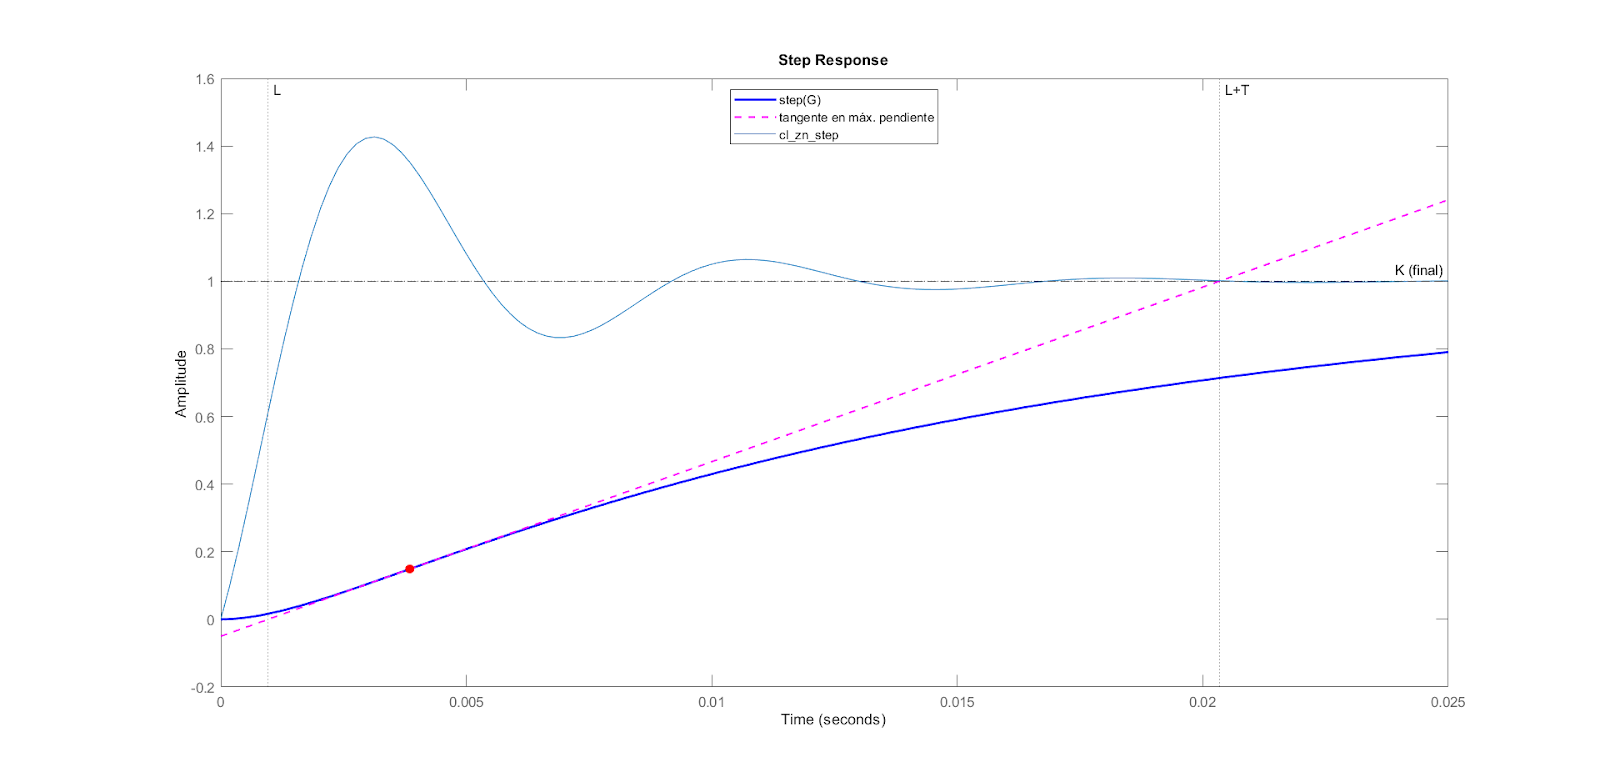
\includegraphics[width=\columnwidth]{img/zn_step_response.png} % <-- coloca aquí tu imagen exportada
	\caption{Respuesta al escalón en lazo abierto con la tangente en el punto de máxima pendiente y la Respuesta al escalon en lazo cerrado usando los valores de \(K_p,T_i\) y \(T_d\) obtenidos por el metodo.}
	\label{fig:zn_step_out}
\end{figure}

\subsubsection*{Cálculo de \(K\), \(L\) y \(T\)}
\begin{itemize}
	\item La ganancia estática del sistema \(K\) se obtiene como el valor final de la salida ante un escalón unitario, es decir \(K = \mathrm{dcgain}(G)\). En nuestro caso, \(K=1\).
	\item El tiempo muerto aparente \(L\) corresponde a la intersección de la tangente (en el punto de máxima pendiente) con el eje tiempo cuando la salida es cero.
	\item La constante aparente \(T\) se obtiene como el tiempo adicional que tarda esa misma tangente en alcanzar el valor final \(K\). Equivalentemente, \(T = K/S\), siendo \(S\) la pendiente máxima.
\end{itemize}

\begin{table}[!t]
	\centering
	\small
	\caption{Reglas de Ziegler--Nichols por respuesta al escalón.}
	\label{tab:zn_rules}
	\resizebox{0.7\columnwidth}{!}{%
		\begin{tabular}{l c c c}
			\toprule
			\textbf{Controlador} & $K_p$ & $T_i$ & $T_d$ \\
			\midrule
		P   & $T/(K\,L)$      & --   & -- \\
		PI  & $0.9\,T/(K\,L)$ & $3L$ & -- \\
		PID & $1.2\,T/(K\,L)$ & $2L$ & $0.5L$ \\
		
			\bottomrule
		\end{tabular}%
	}
\end{table}


Aplicando este método a nuestra planta se encontró:
\[
L = 9.64 \times 10^{-4}~\text{s}, \quad T = 1.94\times 10^{-2}~\text{s}, \quad K=1.
\]
Los parámetros iniciales del PID calculados según Ziegler--Nichols son:
\[
K_p = 24.1, \qquad T_i = 0.00193~\text{s}, \qquad T_d = 0.000482~\text{s}.
\]

En la Figura~\ref{fig:zn_step_out} se muestra la respuesta obtenida con los valores de $K_p$, $T_i$ y $T_d$ calculados. 
Por su parte, en la Tabla~\ref{tab:resultadosPID} se resumen las principales métricas de desempeño del sistema: \emph{overshoot}, tiempo de subida y tiempo de establecimiento.



